\documentclass[a4paper,13pt]{extarticle}
\usepackage[utf8]{inputenc}
\usepackage[english]{babel}
\usepackage{amsmath}
\usepackage{graphicx}
\usepackage{tikz}
\usepackage{geometry}
\usepackage{array}
\usepackage{fancyhdr}
\usepackage{hyperref}
\usepackage{amssymb}
\usepackage{amsfonts}
\usepackage{listings}
\usepackage{xcolor}
\usepackage{csvsimple}
\usepackage[T1]{fontenc}
\usepackage{ragged2e} 
\usepackage[backend=biber,style=numeric]{biblatex}
\addbibresource{references.bib}
\usepackage{setspace} 
\usepackage{algorithm}
\usepackage{pgfplots}
\usepgfplotslibrary{patchplots}
\usepackage{pgfgantt}
\usepackage{array}
\usepackage{booktabs}
\usepackage{longtable}
\usepackage{verbatim}
\usepackage{pgfplots}
\usepackage{tikz-3dplot}
\usepackage{lastpage}
\usepackage{csquotes}
\usepackage{longtable}
\usepackage{framed}  
\addbibresource{references.bib}
\usepackage{enumitem}

\lstset{
    language=C,
    basicstyle=\ttfamily\small, % Font chữ code
    numbers=left,               % Số dòng bên trái
    numberstyle=\tiny\color{gray}, % Style số dòng
    stepnumber=1,               % Đánh số từng dòng
    numbersep=8pt,              % Khoảng cách số dòng và code
    backgroundcolor=\color{white},
    showspaces=false,
    showstringspaces=false,
    showtabs=false,
    frame=single,               % TẠO KHUNG VIỀN (FRAMED)
    rulecolor=\color{black},    % Màu khung
    tabsize=4,
    captionpos=b,
    breaklines=true,
    breakatwhitespace=false,
    title=\lstname,
    keywordstyle=\color{blue},
    commentstyle=\color{green!50!black},
    stringstyle=\color{red}
}

\geometry{
  a4paper,
  total={170mm,257mm},
  left=20mm,
  right=20mm,
  top=20mm,
  bottom=20mm,
}
\renewcommand{\abstractname}{\textbf{\Large\uppercase{Abstract}}}

\everymath{\displaystyle}

\AtBeginDocument{
  \abovedisplayskip=6pt plus 2pt minus 4pt
  \belowdisplayskip=6pt plus 2pt minus 4pt
  \abovedisplayshortskip=0pt plus 2pt
  \belowdisplayshortskip=4pt plus 2pt minus 2pt
}

% Thiết lập header và footer
\pagestyle{fancy}
\fancyhf{} % Xóa các kiểu header và footer mặc định

% Header
\fancyhead[L]{\includegraphics[height=1.5cm]{logobk.png}} 
\fancyhead[C]{\textbf{VIETNAM NATIONAL UNIVERSITY HO CHI MINH CITY\\HO CHI MINH CITY UNIVERSITY OF TECHNOLOGY}}
\fancyhead[R]{}

% Footer
\fancyfoot[C]{\textbf{Page} \thepage\ \textbf{|} \pageref{LastPage}}

\setlength{\headheight}{28pt} % Tăng chiều cao của header để tránh chồng lấn
\setlength{\headsep}{30pt}    % Tạo khoảng cách giữa header và nội dung

% Bỏ header và footer ở trang đầu tiên nếu cần
\renewcommand{\headrulewidth}{0.5pt} % Đường kẻ ở header
\renewcommand{\footrulewidth}{0.5pt} % Đường kẻ ở footer


\begin{document}


\begin{titlepage}
\definecolor{myblue1}{RGB}{3, 43, 145}
\definecolor{myblue2}{RGB}{30, 126, 219}

\begin{tikzpicture}[remember picture, overlay]
  \draw[myblue1, thick] ([shift={(0.8cm, -0.8cm)}]current page.north west) rectangle ([shift={(-0.8cm, 0.8cm)}]current page.south east);
  \draw[myblue2, thick]([shift={(1cm, -1cm)}]current page.north west) rectangle ([shift={(-1cm, 1cm)}]current page.south east);
\end{tikzpicture}

\begin{center}
  \textbf{ VIETNAM NATIONAL UNIVERSITY HO CHI MINH CITY}\\
  \vspace{0.1cm}
  \textbf{HO CHI MINH CITY UNIVERSITY OF TECHNOLOGY}\\
  \vspace{0.1cm}
  \textbf{ FACULTY OF COMPUTER SCIENCE AND ENGINEERING}\\
  \vspace{2.5cm}
      \centering
      \includegraphics[scale = 1.0]{logobk.png} \\
    \vspace{1.0cm}

 \rule{\linewidth}{1pt}      % Dòng kẻ trên (Dày 2pt, dài bằng chiều rộng trang)
  \vspace{0.5cm}              % Khoảng cách giữa dòng kẻ trên và chữ
  
  \textbf{\fontsize{25pt}{0pt}\selectfont PROJECT REPORT}\\
  \vspace{0.5cm}              % Khoảng cách giữa 2 dòng chữ
  \textbf{\LARGE Logic Design Project}\\
  
  \vspace{0.5cm}              % Khoảng cách giữa chữ và dòng kẻ dưới
  \rule{\linewidth}{1pt}      % Dòng kẻ dưới (Dày 2pt)
  
  \vspace{1cm}
    \textbf{TOPIC: SMART GARDENING PROJECT}\\
  \vspace{1cm}
  \textbf{HK251}\\
  \textbf{INSTRUCTOR: M.Eng. NGUYEN THIEN AN}\\
    \vspace{1cm}

  
  {\large
			\begin{tabular}{|c|c|}
				\hline
				\textbf{student's name} & \textbf{Student's ID} \\ \hline
				Nguyen Viet Trung & 2353251 \\ \hline
				Nguyen Hieu Trung & 2353244 \\ \hline
				Nguyen Tam Long   & 2352694 \\ \hline
				Pham Minh Nhat    & 2352863 \\ \hline
				Tran Quoc Thang   & 2353125 \\ \hline
			\end{tabular}
    }
  
  \vspace{4cm}
  \textbf{Ho Chi Minh City, 2025}
\end{center}

\end{titlepage}

\thispagestyle{empty}
\newpage

%%%%%%%%%%%%%%%%%%%%%%%%%%%%%%%%%
\begin{center}
  
    \textbf{ GROUP WORK RESULTS REPORT} \\
    \vspace{0.5cm}
    \begin{tabular}{|c|>{\centering\arraybackslash}m{4cm}|>{\centering\arraybackslash}m{4cm}|>{\centering\arraybackslash}m{3cm}|} \hline
      \textbf{Number} & \textbf{Full name} & \textbf{Student ID} & \textbf{Contribution} \\ \hline
      1 & Nguyen Viet Trung & 2353251 & 100\% \\ \hline
      2 & Nguyen Hieu Trung & 2353244 & 100\% \\ \hline
      3 & Nguyen Tam Long   & 2352694 & 100\% \\ \hline
      4 & Pham Minh Nhat    & 2352863 & 100\% \\ \hline
      5 & Tran Quoc Thang   & 2353125 & 100\% \\ \hline
    \end{tabular} \\
    \end{center}
    
    \vspace{0.5cm}


\newpage

\justifying % Căn đều đoạn văn bản dưới đây
\setstretch{1.5} % Thiết lập khoảng cách giữa các dòng

\tableofcontents
\listoftables
\listoffigures

\clearpage

% ==================================================================
% PART 1: EXECUTIVE & CONTEXT
% ==================================================================

\section{Executive Summary}
\subsection{Goal}
Automate tree washing and irrigation based on real conditions and schedules; reduce human effort; save water versus manual methods; keep foliage clean for better photosynthesis and urban aesthetics.

\subsection{KPIs}
According to the project goals:
\begin{itemize}
    \item High system uptime speed.
    \item Water saving efficiency.
    \item Launching flexibility.
\end{itemize}

\section{Context and Scope}
\subsection{Context and Need}
\begin{itemize}
    \item \textbf{Dusty urban areas:} Require periodic washing of leaves and trunks to improve photosynthesis and appearance.
    \item \textbf{Campuses/parks/farms:} Require irrigation optimized by soil moisture and weather.
\end{itemize}

\subsection{Use Cases}
The system is designed for the following scenarios:
\begin{enumerate}
    \item \textbf{Home Balcony:} 1-4 pots; mini pump + mist nozzles; app on/off; morning/evening schedule; rain skip.
    \item \textbf{Campus/Park:} 10-50 watering points; zoning; per-zone water statistics; alert for low tank/pump jam.
    \item \textbf{Urban washing:} Light-pressure wash cycles at night/off-peak; prioritize cleaning leaves/trunks without wasting water.
\end{enumerate}

\subsection{In Scope \& Out Scope}
\begin{itemize}
    \item \textbf{In scope:} Washing/irrigation automation, remote monitoring, scheduling, alerts, OTA updates, dashboard.
    \item \textbf{Out scope:} Computer vision, autonomous tanker vehicles, automated fertilization (placed on roadmap).
\end{itemize}

\section{System Requirements}
\subsection{Functional Requirements}
The system must fulfill the following functions:
\begin{itemize}
    \item Read sensors: soil moisture, rain, light, flow, ambient temperature/humidity.
    \item Control pump/valves by thresholds, schedule, and manual command from app/web.
    \item Skip washing/irrigation when it rains; stop on detecting leaked water in the dry environment.
    \item Scheduling (cron-like), multi-zone control, manual override with safe timeout.
    \item Log data \& send telemetry (MQTT/HTTPS); buffer when offline.
    \item OTA firmware; remote configuration (Wi-Fi, thresholds, schedules, zones, etc.).
    \item Alert: tank low/dry-run/unusual pressure-flow/disconnect.
\end{itemize}

\subsection{Non-Functional Requirements}
The design adheres to these standards:
\begin{itemize}
    \item Outdoor durability; UV-resistant; waterproof cabling and rust protection.
    \item Security: TLS, key-management, secure boot.
    \item Control latency (delay) $< 2s$ via LAN and $< 5s$ via cloud.
    \item Power: Battery/solar on 12V adapter; deep-sleep, watchdog, auto recovery.
    \item Maintainable: Replace filters/nozzles; check valves/pump; hot-swap node.
\end{itemize}
% ==================================================================
% PART 2: SYSTEM ARCHITECTURE
% ==================================================================

\section{System Architecture}
\subsection{Logic Flow}
The operational logic is defined as follows:
\begin{enumerate}
    \item \textbf{Sensor reading:} Soil moisture, rain detection, light, temperature \& humidity.
    \item \textbf{Condition check:}
    \begin{itemize}
        \item IF soil moisture $<$ threshold (e.g., 40\%).
        \item AND rain sensor indicates "dry".
    \end{itemize}
    \item \textbf{Decision:} ESP32 triggers MOSFET $\rightarrow$ pump ON.
    \item \textbf{Water amount calculation:}
    \begin{equation}
        T_{on} = \frac{V_{water,need}}{Q_{pump}}
    \end{equation}
    Example: $V_{water,need} = 0.6L$, $Q_{pump} = 1.2 L/min \Rightarrow T_{on} = 30s$.
    \item \textbf{Update:} After watering, pump OFF, ESP32 logs data and returns to deep-sleep.
    \item \textbf{Repeat cycle:} Re-check every $T_{check}$ (e.g., 10-15 minutes).
\end{enumerate}

\subsection{Flow Chart}
The overall schematic of the proposed irrigation system includes:
\begin{itemize}
    \item \textbf{Laptop:} Connected via Wi-Fi for monitoring.
    \item \textbf{ESP32:} Central processing unit.
    \item \textbf{LM393 boards:} Interface for sensors.
    \item \textbf{Sensors:} Provide environmental data.
    \item \textbf{Pumping Motor:} Actuator controlled by the system.
\end{itemize}

% ==================================================================
% PART 2: HARDWARE DESIGN
% ==================================================================

\section{Hardware Design}
\subsection{Material}
The following table lists the required components:

\begin{longtable}{p{3cm}p{5cm}p{6cm}}
    \caption{Materials list} \label{tab:bom} \\
    \toprule
    \textbf{Type} & \textbf{Device} & \textbf{Note} \\
    \midrule
    \endfirsthead
    
    \toprule
    \textbf{Type} & \textbf{Device} & \textbf{Note} \\
    \midrule
    \endhead
    
    \bottomrule
    \endfoot

    MCU & ESP32 & Wi-Fi, OTA, TLS \\
    Soil sensor & Soil Moisture Sensor & Active when the soil moisture is over 60 percent.\\
    Rain sensor & Rain Water Sensor & Detect current weather \\
    Temp/Humid & Temperature DHT22/11 & Detect temperature and humidity \\
    Driver & MOSFET (F5305S) & Control the pump \\
    Water Pump & Water Pump 12VDC & Water pumping when matching right conditions \\
    Power & 12V-2A adapter & Maintain the pump anytime \\
\end{longtable}
\subsection{Schematic}
\begin{figure}[H]
    \centering
    \includegraphics[width=0.5\linewidth]{schematic.png}
    \caption{Schematic of the project}
    \label{fig:placeholder}
\end{figure}
\subsection{Calculation}
\subsubsection{Assumption}
Parameters for calculation:
\begin{itemize}
    \item Sources: 
    \begin{itemize}
        \item Pump source: Adapter AC - DC 12 - 2A. So, \(P_{max}=12V \times 2A = 24W\).
        \item MCU source: USB port 5V - 500mA(Wi-Fi activated).
    \end{itemize}
    \item Pump Load (R385):
    \begin{itemize}
        \item Operating voltage: 6 - 12V.
        \item Operating current: 0.5 - 0.7A.
        \item Flow rate: 1-2L/min.
    \end{itemize}
    \item Control load: ESP32 + Sensors:
    \begin{itemize}
        \item Power consumption: 120mA(Wi-Fi activated).
    \end{itemize}
\end{itemize}
\subsubsection{Power margin check}
The power margin of the water pump is calculated to ensure the adapter is not overloaded:
\begin{equation}
    SF = \frac{I_{adapter-max}}{I_{pump}} =  \frac{2.0A}{0.7A} \approx 2.85
\end{equation}
Conclusion: The 12V - 2A adapter is sufficient in this case, operating at approximately 35 percent of its maximum capacity.

Otherwise, the ESP32 is isolated from the pump's power rail, powered directly via USB:
\begin{equation}
    I_{mcu} \approx 120mA < I_{USB-limit} = 500mA
\end{equation}
Conclusion: The USB interface provides ample current for the MCU and sensors, and the physical isolation from the 12V pump circuit prevents potential brownout resets caused by inductive voltage drops.
\subsubsection{Energy consumption estimate}
The daily energy consumption is estimated for operational cost analysis (assuming a standard 10-second watering cycle per day).
\begin{equation}
    E_{total} = E_{control} + E_{pump}
\end{equation}
\begin{itemize}
    \item Control unit:
    \begin{equation}
        E_{control} = 5V \times 0.12A \times 24h = 14.4Wh/day
    \end{equation}
    \item Pump unit:
    \begin{equation}
        E_{pump} = 12V \times 0.7A \times \frac{10}{3600} \approx 0.0233Wh/day
    \end{equation}
    \item Total energy:
    \begin{equation}
        E_{total} = 14.4 + 0.0233 = 14.4233Wh/day
    \end{equation}
\end{itemize}
\subsection{Source code}
\subsubsection{Configuration pin - globalize valuation}

\begin{table}[H]
    \centering
    \caption{ESP32 Pin Configuration}
    \label{tab:pinout}
    \begin{tabular}{ccl}
    \toprule
    \textbf{No.} & \textbf{ESP32 Pin} & \textbf{Device / Note} \\ 
    \midrule
    1 & GPIO 34 & Soil Moisture Sensor (Analog Input) \\
    2 & GPIO 39 & Rain Sensor (Digital Input Only) \\
    3 & GPIO 32 & DHT22 Sensor (Digital I/O) \\
    4 & GPIO 33 & MOSFET (Active High) \\
    \bottomrule
    \end{tabular}
\end{table}
For updating the value for the server, all \(glob\) variables are responsible for this job. \\
In this system, we apply the FreeRTOS, which separates the system into many tasks and manages them with the scheduler. \\
Using a semaphore in the FreeRTOS structure ensures the system executes only one task at a time, which prevents to the wrong input signal for the MCU. 
\begin{lstlisting}
float glob_temp = 0;
float glob_humid = 0;
float glob_soil= 0;
float glob_total_ml = 0;
float glob_rain = 0;
bool glob_pump_running = false;

SemaphoreHandle_t xSensorMutex = NULL;
SemaphoreHandle_t xSerialMutex = NULL;
SemaphoreHandle_t xMqttMutex = NULL;
\end{lstlisting}
\subsubsection{Soil sensor}
\begin{lstlisting}
void soil_sensor(void *pvParameter)
{
    int soil_val = 0;
    int curr_soil_per = 0;

    while (1)
    {
        soil_val = analogRead(SOIL_PIN);

        curr_soil_per = map(soil_val, 4095, 0, 0, 100);

        if (xSensorMutex != NULL &&
            xSemaphoreTake(xSensorMutex, portMAX_DELAY) == pdTRUE)
        {
            glob_soil = curr_soil_per;
            xSemaphoreGive(xSensorMutex);
        }
        vTaskDelay(pdMS_TO_TICKS(2000));
    }
}
\end{lstlisting}
\subsubsection{Humidity anđ temperature sensor}
\begin{lstlisting}
void temp_humid_sensor(void *pvParameter)
{
    dht.begin();

    float current_temp = 0;
    float current_humid = 0;
    while (1)
    {
        current_temp = dht.readTemperature();
        current_humid = dht.readHumidity();
        if (xSensorMutex != NULL &&
            xSemaphoreTake(xSensorMutex, portMAX_DELAY) == pdTRUE)
        {
            glob_temp = current_temp;
            glob_humid = current_humid;
            xSemaphoreGive(xSensorMutex);
        }
        vTaskDelay(pdMS_TO_TICKS(2000));
    }
}
\end{lstlisting}
\subsubsection{Rain sensor}
\begin{lstlisting}
void rain_sensor(void *pvParameter)
{
    pinMode(RAIN_PIN, INPUT);

    while (1)
    {
        int rain_value = analogRead(RAIN_PIN);
        if (xSensorMutex != NULL &&
            xSemaphoreTake(xSensorMutex, portMAX_DELAY) == pdPASS)
        {
            glob_rain = rain_value;
            xSemaphoreGive(xSensorMutex);
        }
        vTaskDelay(pdMS_TO_TICKS(2000));
    }
}
\end{lstlisting}
\subsubsection{WI-FI connection}
To use the system wirelessly, we implement the task WiFi to control the MCU anđ check them every 5 second. 
\begin{lstlisting}
void task_WiFi(void *pvParameter)
{

    bool logged = false;

    while (1)
    {
        if (WiFi.status() != WL_CONNECTED)
        {
            logged = false;

            if (xSerialMutex != NULL &&
                xSemaphoreTake(xSerialMutex, portMAX_DELAY) == pdPASS)
            {
                Serial.print("WiFi not connected, start connecting");
                WiFi_Connect();
                xSemaphoreGive(xSerialMutex);
            }
        }
        else if (!logged)
        {
            if (WiFi.status() == WL_CONNECTED)
            {
                if (xSerialMutex != NULL &&
                    xSemaphoreTake(xSerialMutex, portMAX_DELAY) == pdPASS)
                {
                    Serial.print("WiFi connected, IP: ");
                    Serial.println(WiFi.localIP());
                    xSemaphoreGive(xSerialMutex);
                }
            }

            logged = true;
        }
        else if (logged)
        {
            if (xSerialMutex != NULL &&
                xSemaphoreTake(xSerialMutex, portMAX_DELAY) == pdPASS)
            {
                Serial.println("WiFi still connected");
                xSemaphoreGive(xSerialMutex);
            }
        }

        vTaskDelay(pdMS_TO_TICKS(5000));
    }
}
\end{lstlisting}

% ==================================================================
% PART 3: ENCRYPTION
% ==================================================================

\section{Detailed Implementation and Security}
This section expands on the general design with specific technical details regarding hardware connections, communication protocols, and security measures.



\subsection{SHA-256 Data Encoding Module}

\subsubsection{Overview}
The following module is responsible for collecting five floating-point sensor values, serializing them into a 20-byte buffer, hashing that buffer using the SHA-256 algorithm (from the mbedTLS library), and finally producing a 52-byte output. The output consists of the raw input data followed by the computed hash digest:

\[
\text{output52} = \text{input[20]} \parallel \text{digest[32]}
\]

This design makes it possible to transmit the original sensor data together with a hash-based integrity check.

\subsubsection{Source Code}

\begin{lstlisting}
uint8_t output52[52];

void sha2(float temp, float hum, float soid, float total_ml, float rain){
    uint8_t input[20];

    memcpy(input + 0,  &temp,     4);
    memcpy(input + 4,  &hum,      4);
    memcpy(input + 8,  &soid,     4);
    memcpy(input + 12, &total_ml, 4);
    memcpy(input + 16, &rain,     4);

    uint8_t out32[32];

    mbedtls_sha256_context ctx;
    mbedtls_sha256_init(&ctx);
    mbedtls_sha256_starts_ret(&ctx, 0);
    mbedtls_sha256_update_ret(&ctx, input, 20);
    mbedtls_sha256_finish_ret(&ctx, out32);

    memcpy(output52,      input, 20);
    memcpy(output52 + 20, out32, 32);
}
\end{lstlisting}

\subsubsection{Function Explanation}

\begin{itemize}
    \item Five floating-point values are packed into a 20-byte array using \texttt{memcpy}, each occupying 4 bytes (IEEE-754 binary representation).
    \item The SHA-256 hashing context is initialized, updated with the 20 bytes of input, and finalized to produce a 32-byte digest.
    \item The final output array is formed by concatenating:
          \begin{enumerate}
              \item the original 20 bytes of raw input data,
              \item the 32-byte SHA-256 hash digest.
          \end{enumerate}
    \item The resulting 52-byte buffer can be transmitted or stored for later verification.
\end{itemize}

\subsubsection{Data Flow Diagram}

\[
\underbrace{4B_{temp} + 4B_{hum} + 4B_{soil} + 4B_{total\_ml} + 4B_{rain}}_{\text{20 bytes input}}
\quad \xrightarrow{\text{SHA-256}} \quad
\text{digest (32 bytes)}
\]

\[
\text{output52} = \boxed{\text{input (20B)}} \;||\; \boxed{\text{SHA-256 digest (32B)}}
\]

\subsubsection{Notes and Considerations}

\begin{itemize}
    \item The floats are hashed in their raw binary form, meaning the output may vary across platforms with different endianness. For cross-platform reproducibility, data should be normalized (e.g., convert to big-endian or text representation).
    \item SHA-256 provides integrity but \textbf{not encryption}. The original data is still readable.
    \item For authentication (preventing forgery), the system should use HMAC-SHA256 with a secret key.
    \item Error checking and \verb|mbedtls_sha256_free| are recommended for robustness in production code.
\end{itemize}

\subsection{Task Synchronization using Semaphore \& Mutex}

In a multi-tasking FreeRTOS environment, sensor acquisition, control logic,
and communication processes run concurrently on the ESP32. Without proper
synchronization, shared variables such as temperature, humidity or soil
moisture could be read at the same time they are written, leading to
corrupted values, unstable control behavior or wrong telemetry packets.

To guarantee safe data sharing between tasks, the system applies
\textbf{mutex / binary semaphore} mechanisms:

\begin{itemize}
    \item \textbf{xSensorMutex} – protects access to global sensor data 
          \verb|glob_temp, glob_humid, glob_soil, glob_rain|.
    \item \textbf{xSerialMutex} – mutex for serial console printing to avoid
          overlapped or interleaved logs.
    \item \textbf{xMqttMutex} – ensures only one MQTT publish routine executes
          at a time, preventing memory corruption during JSON serialization.
    \item \textbf{xPumpMutex} – serializes access to the pump so that only one
          watering session (automatic or manual) can run at a time.
\end{itemize}

\textbf{Reasons for using mutexes:}
\begin{enumerate}
    \item Prevent race conditions between sensor tasks updating values simultaneously.
    \item Ensure atomic reads when the MQTT task accesses shared data for publishing.
    \item Avoid serial-output corruption caused by concurrent print calls.
    \item Guarantee exclusive control over pump start/stop logic.
\end{enumerate}

\subsubsection{Data Flow Model with Mutex Protection}

\begin{figure}[H]
\centering
% Bắt đầu co giãn
\resizebox{\textwidth}{!}{%
    \begin{tikzpicture}[
        box/.style={
            rectangle, rounded corners,
            minimum width=4.3cm,
            minimum height=1.1cm,
            draw=black, thick,
            align=center,
            font=\normalsize
        },
        arrow/.style={->, thick},
        node distance=3.2cm and 2.5cm
    ]

    \node[box] (sensor) {Sensor Tasks\\(Soil, Temp/Humid, Rain)};

    \node[box, right=3.5cm of sensor] (shared)
        {Shared Global Variables\\
         \texttt{glob\_temp, glob\_soil,\dots}\\
         Protected by \textbf{xSensorMutex}};

    \node[box, above right=1.5cm and 2.7cm of shared] (mqtt)
        {MQTT Task\\Telemetry Publish};

    \node[box, below right=1.5cm and 2.7cm of shared] (pump)
        {Pump Control\\(in MQTT callback)\\
         Protected by \textbf{xPumpMutex}};

    \draw[arrow] (sensor) -- (shared);
    \draw[arrow] (shared) -- (mqtt);
    \draw[arrow] (shared) -- (pump);

    \end{tikzpicture}%
} % Kết thúc co giãn
\caption{Mutex-based data flow between sensor tasks, shared state, telemetry and pump control}
\label{fig:mutex-flow}
\end{figure}


Shared global data is only accessed when the mutex is locked:

\begin{lstlisting}
// Write (Sensor Task)
if (xSemaphoreTake(xSensorMutex, portMAX_DELAY) == pdTRUE) {
    glob_temp  = current_temp;
    glob_humid = current_humid;
    glob_soil  = current_soil;
    glob_rain  = current_rain;
    xSemaphoreGive(xSensorMutex);
}

// Read (MQTT Task or Pump Control Path)
if (xSemaphoreTake(xSensorMutex, portMAX_DELAY) == pdTRUE) {
    float t = glob_temp;
    float h = glob_humid;
    float s = glob_soil;
    float r = glob_rain;
    xSemaphoreGive(xSensorMutex);
}
\end{lstlisting}

\subsubsection{Pump Control and Mutual Exclusion}

Pump operation is exposed through a small hardware abstraction layer:
\verb|pump_init()|, \verb|pump_start(durationMs, mode)|,
\verb|pump_stop(runTimeMs)| and \verb|pump_set_mode(mode)|. These
functions drive \verb|PUMP_PIN| and update global state
(\verb|glob_pump_running|); all concurrency guarantees are enforced at
the task level.

In the current implementation, all pump commands originate from the MQTT
callback. The downlink payload is a fixed-length binary frame; after
SHA-256 verification, three fields are decoded:

\begin{figure}[H]
\centering
\begin{tikzpicture}[
    box/.style={
        rectangle, rounded corners,
        minimum width=3.8cm,       % Chiều rộng vừa phải
        minimum height=1.2cm,
        draw=black, thick,
        align=center,
        font=\small                % Giảm font một chút
    },
    arrow/.style={->, thick, >=stealth},
    node distance=1.0cm and 1.0cm  % Khoảng cách dọc và ngang
]

% --- Hàng 1: Từ trái qua phải ---
\node[box] (cloud) {Mobile App /\\Web Dashboard};
\node[box, right=of cloud] (broker) {MQTT Broker};
\node[box, right=of broker] (mqtt) {MQTT Task\\parse + SHA-256 verify};

% --- Hàng 2: Xuống dòng và đi ngược lại ---
\node[box, below=of mqtt] (pump) {Pump Control\\guarded by \textbf{xPumpMutex}};
\node[box, left=of pump] (act) {Pump Driver\\MOSFET $\rightarrow$ R385};

% --- Vẽ mũi tên ---
\draw[arrow] (cloud) -- (broker);
\draw[arrow] (broker) -- (mqtt);
\draw[arrow] (mqtt) -- (pump); % Mũi tên đi xuống
\draw[arrow] (pump) -- (act);  % Mũi tên sang trái

\end{tikzpicture}
\caption{Command execution path for manual/remote pump control}
\label{fig:command-path}
\end{figure}

Before calling \verb|pump_start| or \verb|pump_stop|, the callback must
take \verb|xPumpMutex|. Only when the mutex is acquired will the pump
state and mode be changed:

\begin{lstlisting}
// Inside mqttCallback after hash verification
if (xPumpMutex != NULL &&
    xSemaphoreTake(xPumpMutex, portMAX_DELAY) == pdPASS)
{
    if (pump_control == 1) {
        pump_start(duration * 1000, mode);
    } else if (pump_control == 0) {
        pump_stop(duration);
    }

    pump_set_mode(mode);
    xSemaphoreGive(xPumpMutex);
}
else
{
    Serial.println("[MQTT] Cannot take xPumpMutex, command ignored");
}
\end{lstlisting}

This design ensures that:
\begin{itemize}
    \item Only one pump command sequence is active at a time, even if
          future automatic tasks are added.
    \item Manual commands cannot overlap and generate conflicting ON/OFF
          transitions on the motor.
    \item The actuation path (MQTT callback $\rightarrow$ pump driver) is
          deterministic and free of race conditions.
\end{itemize}

\subsubsection{Secure Command Path Flow}

\begin{figure}[H]
\centering
\begin{tikzpicture}[
    box/.style={
        rectangle, rounded corners,
        minimum width=3.5cm,
        minimum height=1.2cm,
        draw=black, thick,
        align=center,
        font=\small
    },
    arrow/.style={->, thick, >=stealth}, % Thêm >=stealth cho mũi tên đẹp hơn
    node distance=1.0cm and 2.0cm        % Khoảng cách dọc và ngang
]

% --- HÀNG 1: Mobile -> Broker -> MQTT Task ---
\node[box] (cloud) {Mobile App /\\Web Dashboard};
\node[box, right=of cloud] (broker) {MQTT Broker};
\node[box, right=of broker] (mqtt) {MQTT Task\\parse + SHA-256 verify};

% --- HÀNG 2: Pump Control -> Pump Driver (Nằm dưới và lùi về trái) ---
\node[box, below=of mqtt] (pump) {Pump Control\\guarded by \textbf{xPumpMutex}};
\node[box, left=of pump] (act) {Pump Driver\\MOSFET $\rightarrow$ R385};

% --- VẼ MŨI TÊN ---
% 1. Cloud -> Broker
\draw[arrow] (cloud) -- node[above,font=\footnotesize]{Publish cmd} (broker);

% 2. Broker -> MQTT
\draw[arrow] (broker) -- node[above,font=\footnotesize]{Payload} (mqtt);

% 3. MQTT -> Pump (Đi xuống)
\draw[arrow] (mqtt) -- node[right,font=\footnotesize, align=left]{Valid hash\\Take Mutex} (pump);

% 4. Pump -> Actuator (Đi sang trái)
\draw[arrow] (pump) -- node[above,font=\footnotesize]{Drive GPIO} (act);

\end{tikzpicture}
\caption{Command execution path for manual/remote pump control}
\label{fig:command-path}
\end{figure}

The downlink command must pass several safety layers:

\begin{enumerate}
    \item The mobile/web client sends a binary control frame through the
          MQTT broker.
    \item The ESP32 MQTT task receives the payload and recomputes the
          SHA-256 hash to verify integrity.
    \item If the hash is valid, the task attempts to acquire
          \verb|xPumpMutex| and, if successful, executes
          \verb|pump_start| or \verb|pump_stop| and updates the mode.
    \item If the hash check fails or the mutex cannot be acquired, the
          command is rejected safely and the current watering session
          continues unaffected.
\end{enumerate}

\paragraph{Conclusion}
By implementing semaphore–mutex protection, communication between
sensing tasks, communication tasks and the pump actuator is safe,
atomic and deadlock-free. Data integrity during MQTT uplink and
exclusive access to the pump during downlink commands are preserved,
ensuring reliable cloud monitoring and stable irrigation execution.


\subsection{MQTT Module Overview}
The MQTT Task (\texttt{taskMqtt}) is a critical component responsible for Internet of Things (IoT) connectivity. It abstracts the complexities of the TCP/IP stack and the MQTT protocol, providing a seamless interface for control and monitoring.

\textbf{Key Responsibilities:}
\begin{itemize}
    \item \textbf{Connectivity Management:} Automatically establishes and maintains Wi-Fi and MQTT connections.
    \item \textbf{Telemetry Uplink:} Periodically aggregates sensor data (Temperature, Humidity, Soil Moisture, Rain) and publishes it to the cloud.
    \item \textbf{Command Downlink:} Listens for remote control commands to operate the water pump.
    \item \textbf{Security:} Implements SHA-256 hashing to verify the integrity and authenticity of received commands.
\end{itemize}

\subsubsection{System Configuration \& Dependencies}

\paragraph{Library Dependencies}
The module relies on the following standard and custom libraries:
\begin{table}[H]
    \centering
    \begin{tabular}{|l|l|}
        \hline
        \textbf{Library} & \textbf{Purpose} \\ \hline
        \texttt{WiFi.h} & Manages the physical layer and IP stack connection. \\ \hline
        \texttt{PubSubClient.h} & A lightweight client for simple MQTT communication. \\ \hline
        \texttt{ArduinoJson.h} & Efficient serialization/deserialization of JSON data. \\ \hline
        \texttt{mbedtls/sha256.h} & Hardware-accelerated cryptographic hashing. \\ \hline
        \texttt{pump\_control.h} & Hardware abstraction layer for the water pump. \\ \hline
    \end{tabular}
    \caption{Library Dependencies}
\end{table}

\paragraph{Network Configuration}
The system connects to a public broker for demonstration purposes but is designed to be broker-agnostic.
\begin{itemize}
    \item \textbf{Broker Address:} \texttt{broker.hivemq.com}
    \item \textbf{Port:} 1883 (Non-SSL)
    \item \textbf{Topics:}
    \begin{itemize}
        \item \textbf{Sensor Data (Pub):} \texttt{device/sensor/data}
        \item \textbf{Command (Sub):} \texttt{device/command}
    \end{itemize}
\end{itemize}

\subsubsection{Secure Command Protocol (Downlink)}
To prevent unauthorized or corrupted commands from triggering the actuators, the system employs a \textbf{Binary Protocol with SHA-256 Verification}. This is defined under the \texttt{NON\_ENCRYPTION} macro in the source code.

\paragraph{Packet Structure}
The incoming payload must be at least \textbf{38 bytes} long. The structure is defined as follows:

\begin{table}[H]
    \centering
    \begin{tabular}{|c|c|c|l|}
        \hline
        \textbf{Offset} & \textbf{Size} & \textbf{Type} & \textbf{Description} \\ \hline
        0 & 1 Byte & \texttt{uint8\_t} & \textbf{Pump Control}: 1 (Start), 0 (Stop). \\ \hline
        1 & 4 Bytes & \texttt{uint32\_t} & \textbf{Duration}: Runtime in seconds (Little Endian). \\ \hline
        5 & 1 Byte & \texttt{uint8\_t} & \textbf{Mode}: 0 (Manual), 1 (Automatic). \\ \hline
        6 & 32 Bytes & \texttt{uint8\_t[]} & \textbf{SHA-256 Hash}: Integrity signature. \\ \hline
    \end{tabular}
    \caption{Binary Command Packet Structure}
\end{table}

\paragraph{Integrity Verification Logic}
Upon receiving a message, the \texttt{mqttCallback} function performs the following validation steps:
\begin{enumerate}
    \item \textbf{Length Check:} Discards packet if \texttt{len < 38}.
    \item \textbf{Extraction:} Separates the data payload (Bytes 0-5) from the received hash (Bytes 6-37).
    \item \textbf{Hashing:} Uses \texttt{mbedtls\_sha256} to calculate the hash of the first 6 bytes.
    \item \textbf{Comparison:} Compares the calculated hash with the received hash using \texttt{memcmp}.
    \item \textbf{Execution:} 
    \begin{itemize}
        \item If hashes match: The pump state is updated via \texttt{pump\_start()} or \texttt{pump\_stop()}.
        \item If mismatch: Prints "HASH FAILED" and ignores the command.
    \end{itemize}
\end{enumerate}


\subsubsection{Telemetry Protocol (Uplink)}
The system publishes sensor data using \textbf{JSON format} for high compatibility with web dashboards and databases.

\paragraph{Data Aggregation \& Hashing}
Before serialization, the system aggregates 5 sensor values (20 bytes total) and calculates a SHA-256 hash. This hash is stored in a global buffer \texttt{output52} for potential future verification features.

\textbf{Input Data Map:}
\begin{itemize}
    \item Bytes 0-3: Temperature (float)
    \item Bytes 4-7: Humidity (float)
    \item Bytes 8-11: Soil Moisture (float)
    \item Bytes 12-15: Total Water Volume (float)
    \item Bytes 16-19: Rain Status (float)
\end{itemize}

\paragraph{JSON Serialization}
The \texttt{ArduinoJson} library is used to format the payload. The \texttt{serialized()} function is employed to format floating-point numbers to exactly 2 decimal places, optimizing the string length.

\textbf{Example Payload:}
\begin{verbatim}
{
  "temp": 28.50,
  "hum": 65.20,
  "soil": 45.00,
  "rain": 0.00,
  "water_ml": 1200.50
}
\end{verbatim}

\subsubsection{Task Implementation Details}
The module runs as a FreeRTOS task, ensuring non-blocking operation alongside other system components.

\paragraph{Initialization Phase}
\begin{itemize}
    \item \textbf{Pump Init:} Configures GPIO pins for the relay/motor driver.
    \item \textbf{MQTT Setup:} Configures the Broker URL, Port, and Callback function.
\end{itemize}

\paragraph{Main Loop Logic}
The task executes the following operations in a continuous loop:



[Image of MQTT architecture diagram]


\begin{enumerate}
    \item \textbf{Connection Maintenance:}
        \begin{itemize}
            \item Checks Wi-Fi status. If disconnected, waits 2 seconds.
            \item Checks MQTT status. If disconnected, attempts to reconnect using a random Client ID to prevent session conflicts.
        \end{itemize}
    
    \item \textbf{Keep-alive:} Calls \texttt{s\_mqttClient.loop()} to handle incoming packets (PINGRESP, PUBLISH).
    
    \item \textbf{Sensor Data Acquisition:}
        \begin{itemize}
            \item Uses \texttt{xSemaphoreTake(xSensorMutex)} to safely read global variables updated by the Sensor Task.
            \item This prevents race conditions where data might be read while being written.
        \end{itemize}
    
    \item \textbf{Data Sanitization:} Checks for \texttt{NaN} (Not a Number) values and resets them to 0.0 to prevent JSON errors.
    
    \item \textbf{Publishing:} Serializes the data and publishes it to \texttt{TOPIC\_SENSOR}.
    
    \item \textbf{Timing:} Uses \texttt{vTaskDelayUntil} for a precise 5-second sampling interval.
\end{enumerate}

% ==================================================================
% PART 2: SOFTWARE SYSTEM
% ==================================================================

\section{Software System}
\subsection{Backend Logic}
The backend is built using \textbf{Node.js} with the \textbf{Express} framework, offering non-blocking I/O suitable for real-time IoT applications. It serves as the bridge between the frontend dashboard, the AI service, and the MQTT broker.

The server maintains the system state in memory and uses \texttt{socket.io} to push real-time updates to connected clients.

\begin{lstlisting}[language=Java, caption={Server State Management (server.js)}, label={lst:serverstate}]
// System state
let systemState = {
  pumpOn: false,
  mode: 'automatic', // 'automatic' or 'manual'
  pumpStartTime: null,
  pumpDuration: 0,
  aiEnabled: process.env.AI_ENABLED !== 'false',
  lastAIDecision: null
};

// Listen for sensor updates via MQTT
mqttClient.on('message', (topic, message) => {
    // ... parse data ...
    io.emit('sensor_update', sensorData);
});
\end{lstlisting}

\subsection{AI Decision Service}

In the architecture of the smart watering system, the \textbf{AI Decision Service} subsystem plays the role of a central processing unit. It is responsible for analyzing real-time environmental parameters and making automated pump control decisions (ON/OFF), replacing traditional rigid control rules.

\subsubsection{Theoretical Background}

To address the binary classification problem for irrigation decisions, the team selected the \textbf{Random Forest} algorithm.

\paragraph{Algorithm Theory:}
Random Forest is a machine learning method belonging to the \textit{Ensemble Learning} group. Instead of building a single Decision Tree, Random Forest constructs a collection (forest) consisting of multiple decision trees during the training process.
\begin{itemize}
    \item \textbf{Operation Mechanism:} Each tree in the forest outputs an individual prediction (e.g., "Water" or "Do not water"). The final result of the model is determined based on the \textit{Voting} mechanism (majority vote) from all individual trees.
    \item \textbf{Bagging \& Random Subspace:} The algorithm utilizes Bootstrap Aggregating techniques to create random subsets of data for each tree, which enhances diversity and the stability of the model.
\end{itemize}

\paragraph{Justification for Selection:}
Compared to other algorithms such as Neural Networks (RNN/LSTM) or a Single Decision Tree, Random Forest was chosen because:
\begin{enumerate}
    \item \textbf{High Accuracy:} It overcomes the \textit{Overfitting} drawback commonly found in single decision trees.
    \item \textbf{Suitability for Tabular Data:} The system's input data consists of discrete fields (Temperature, Humidity, Soil Moisture) and does not require sequential time-series processing like RNN/LSTM.
    \item \textbf{Low Computational Cost:} It offers fast inference speeds, making it suitable for embedded integration or running on servers with limited resources.
\end{enumerate}

\subsubsection{Data Processing \& Training}

\paragraph{1. Data Source:}
Due to time constraints in the project implementation, collecting real-world data on crops over a long period was not feasible. The team utilized the standard \textbf{Tomato Irrigation Dataset} from the Mendeley research data repository\footnote{\url{https://data.mendeley.com/datasets/33cngpcrmx/2}}. This dataset records experimental environmental parameters affecting the growth of tomato plants.

\paragraph{2. Data Preprocessing:}
The raw initial data contained many parameters incompatible with the current hardware (such as Nitrogen, Potassium levels, pH...). The processing was performed via the \texttt{pre\_train.py} script with the following steps:

\begin{itemize}
    \item \textbf{Cleaning and Renaming:} Removed trailing whitespace and normalized column names for easier manipulation.
    \item \textbf{Feature Selection:} Extracted only the 3 parameters corresponding to the system's sensors:
    \begin{lstlisting}[language=Python]
# pre_train.py - Lines 8-12
selected_columns = ['Temperature [_ C]', 'Humidity [%]', 'Soil moisture']
df_clean = df[selected_columns].copy()
df_clean.columns = ['temp', 'hum', 'soil']
    \end{lstlisting}
    
    \item \textbf{Data Labeling:} 
    Since the original dataset lacked a pump decision column (Label), the team applied agricultural logic to automatically generate the \texttt{Pump\_Action} label. This logic includes 3 priority condition branches to optimize watering:
    \begin{lstlisting}[language=Python]
# pre_train.py - Lines 15-24: Label generation logic
def generate_label(row):
    # 1. Soil too dry (<350) -> Pump immediately
    if row['soil'] < 350: 
        return 1
    # 2. Hot weather (>30 C) and soil starting to dry -> Pump to prevent heat shock
    elif row['temp'] > 30 and row['soil'] < 450:
        return 1
    # 3. Dry air (<50%) -> Pump to compensate for transpiration
    elif row['hum'] < 50 and row['soil'] < 550:
        return 1
    else:
        return 0
    \end{lstlisting}
\end{itemize}
The processed result was saved as \texttt{dataset\_chuan.csv} to serve the training process.

\paragraph{3. Model Training:}
The training process was executed in the \texttt{training.py} file using the \texttt{scikit-learn} library.

\begin{itemize}
    \item \textbf{Data Splitting:} The data was split into 80\% for Training and 20\% for Testing.
    \item \textbf{Hyperparameters:} Configured \texttt{RandomForestClassifier} with 100 decision trees (\texttt{n\_estimators=100}) and a maximum depth of 10 (\texttt{max\_depth=10}) to balance complexity and performance.
    \begin{lstlisting}[language=Python]
# training.py - Lines 17-20
X_train, X_test, y_train, y_test = train_test_split(X, y, test_size=0.2, random_state=42)

print("training Random Forest...")
clf = RandomForestClassifier(n_estimators=100, max_depth=10, random_state=42)
clf.fit(X_train, y_train)
    \end{lstlisting}
    \item \textbf{Evaluation:} The model achieved an accuracy of approximately \textbf{99.83\%} on the test set, with Precision and Recall metrics reaching maximum levels for both label classes (0 and 1).
    \item \textbf{Serialization:} The trained model was serialized into a \texttt{model\_tuoi\_cay.pkl} file using the \texttt{joblib} library for reuse.
\end{itemize}

\subsubsection{Model Integration into Backend}

To integrate AI capabilities into the Node.js Web system, the team utilized a \textbf{Child Process} mechanism to create a communication bridge between the Node.js and Python environments.

\paragraph{1. Python AI Service:}
An independent Python script (\texttt{AI\_service.py}) was built to load the \texttt{.pkl} model and perform predictions upon invocation. This script accepts input parameters via command-line arguments and returns the result in JSON format.

\begin{lstlisting}[language=Python]
model = joblib.load('.../backend/model_tuoi_cay.pkl')

# Receive arguments from Node.js (sys.argv)
temp = float(sys.argv[1])
humid = float(sys.argv[2])
soil = float(sys.argv[3])

# Create DataFrame and Predict
iinput_data = pd.DataFrame([[temp, humid, (soil + 1)*50]], 
                              			columns=['temp', 'hum', 'soil'])
prediction = model.predict(input_data)

# Return JSON result
result = {
    "action": int(prediction[0]), 
    "reason": "AI Model Decision"
}
print(json.dumps(result))
\end{lstlisting}

\paragraph{2. Invoking AI from Node.js Server:}
Whenever the server receives new sensor data via the MQTT protocol, it triggers the prediction process. The \texttt{askPythonAI} function executes the Python script, passing the \texttt{temp, hum, soil} parameters, and awaits the returned result to control the device.

This workflow ensures the decoupling of the Server's business logic and the AI's processing logic, facilitating easy maintenance and upgrades.

\subsection{Frontend Web Dashboard}
The user interface is developed using \textbf{ReactJS} and styled with Tailwind CSS. It provides a comprehensive view of the garden's status and allows for manual intervention. Key components include:

\begin{enumerate}
    \item \textbf{SmartWateringDashboard.jsx:} The main controller that connects to the WebSocket to display real-time sensor gauges (Temperature, Humidity, Soil) and pump status.
    \item \textbf{History.jsx:} A log viewer that stores watering events (timestamp, duration, water volume) in local storage and allows CSV export.
    \item \textbf{ConfirmStopPage.jsx:} A safety mechanism that requires user confirmation before interrupting an active watering cycle.
\end{enumerate}

\begin{lstlisting}[language=Java, caption={Real-time Dashboard Logic (SmartWateringDashboard.jsx)}, label={lst:dashboard}]
useEffect(() => {
    // Connect to WebSocket
    websocketService.connect();

    // Handle sensor updates from WebSocket
    const handleSensorUpdate = (data) => {
      setSensors({
        temp: data.temp || 0,
        hum: data.hum || 0,
        soil: data.soil || 0,
        level: data.level || 0,
        // ...
      });
    };

    websocketService.on('sensor_update', handleSensorUpdate);
    websocketService.on('status_update', handleStatusUpdate);
    
    return () => { /* cleanup */ };
}, []);
\end{lstlisting}

\newpage
\section{Estimated Cost}
The following table provides a cost estimation for building a single hardware node:

\begin{table}[H]
    \centering
    \caption{Component Cost Estimation (1 Node)}
    \label{tab:cost}
    \begin{tabular}{clcr}
    \toprule
    \textbf{No.} & \textbf{Component Name} & \textbf{Qty} & \textbf{Total (VND)} \\ 
    \midrule
    1 & ESP32-NodeMCU-32S CH340 Ai-Thinker & 1 & 190.000 \\
    2 & Soil Moisture Sensor & 1 & 12.000 \\
    3 & Rain Water Sensor & 1 & 11.000 \\
    4 & DHT22 Temperature Humidity Sensor & 1 & 103,000 \\
    5 & MOSFET F5305S & 1 & 21.000 \\
    6 & Water Pump R385(12V) & 1 & 47.000 \\
    7 & Power Adapter 12V-2A & 1 & 65.000 \\
    8 & Waterproof Enclosure & 1 & 50.000 \\
    9 & Accessories (Wires, Tubing, Nozzles) & 1 & 50.000 \\
    \midrule
    \multicolumn{3}{r}{\textbf{TOTAL}} & \textbf{549,000} \\ 
    \bottomrule
    \end{tabular}
\end{table}

\section{Conclusion}
The Smart Gardening Project has been successfully designed from high-level logic down to specific hardware and software components. By combining robust hardware (ESP32, weatherproof sensors) with intelligent software (Fuzzy Logic, MQTT with Encryption), the system addresses the critical needs of urban and agricultural irrigation, ensuring water efficiency and operational reliability.

\section{Source Code}

\end{document}





